%%%%%%%%%%%%%%%%%%%%%%%%%%%%%%%%%%%%%%%%%%%%%%%%%%%
%																													
%																												
%																													
%									Importations	de bibliothèques	
%																													
%																												
%%%%%%%%%%%%%%%%%%%%%%%%%%%%%%%%%%%%%%%%%%%%%%%%%%%


\documentclass[hidelinks]{article}
\usepackage[utf8]{inputenc}
\usepackage{graphicx}
\usepackage[T1]{fontenc}
\usepackage[french]{babel}
\usepackage{csquotes}
\usepackage[section]{placeins}
\usepackage{tikz}
\usepackage{hyperref}
\usepackage{afterpage}
\usepackage{pdfpages}
\usepackage{wrapfig}
\usepackage{amsmath, mathtools}
\usepackage{amssymb}
\usepackage{fancyhdr}
\usepackage[all]{background}


%%%%%%%%%%%%%%%%%%%%%%%%%%%%%%%%%%%%%%%%%%%%%%%%%%%%%%%%%%%%%%%%%%%%
%																																	   %
%																																	   %
%																																	   %
%															Page de garde															   %
%																																	   %
%																																	   %
%%%%%%%%%%%%%%%%%%%%%%%%%%%%%%%%%%%%%%%%%%%%%%%%%%%%%%%%%%%%%%%%%%%%



\newcommand{\MyGraphicLogo}{% For imported graphic logo
\begin{tikzpicture}[remember picture,overlay,yshift=-15cm, xshift=10.5cm]
	\definecolor{gris}{RGB}{16,52,78}
	\definecolor{jaune_fonce}{RGB}{0, 107, 163}
	\definecolor{jaune}{RGB}{0, 151, 136}
	\fill [gris] (-10.5,-10) -- (0,-4.5) -- (14,-13) -- (14,-16)--(0,-16)--(-10.5,-16);
	\fill [jaune_fonce] (0,-4.5) -- (-10.5,-10) -- (-10.5, 1.8);
	\node at (3.8,0.4) {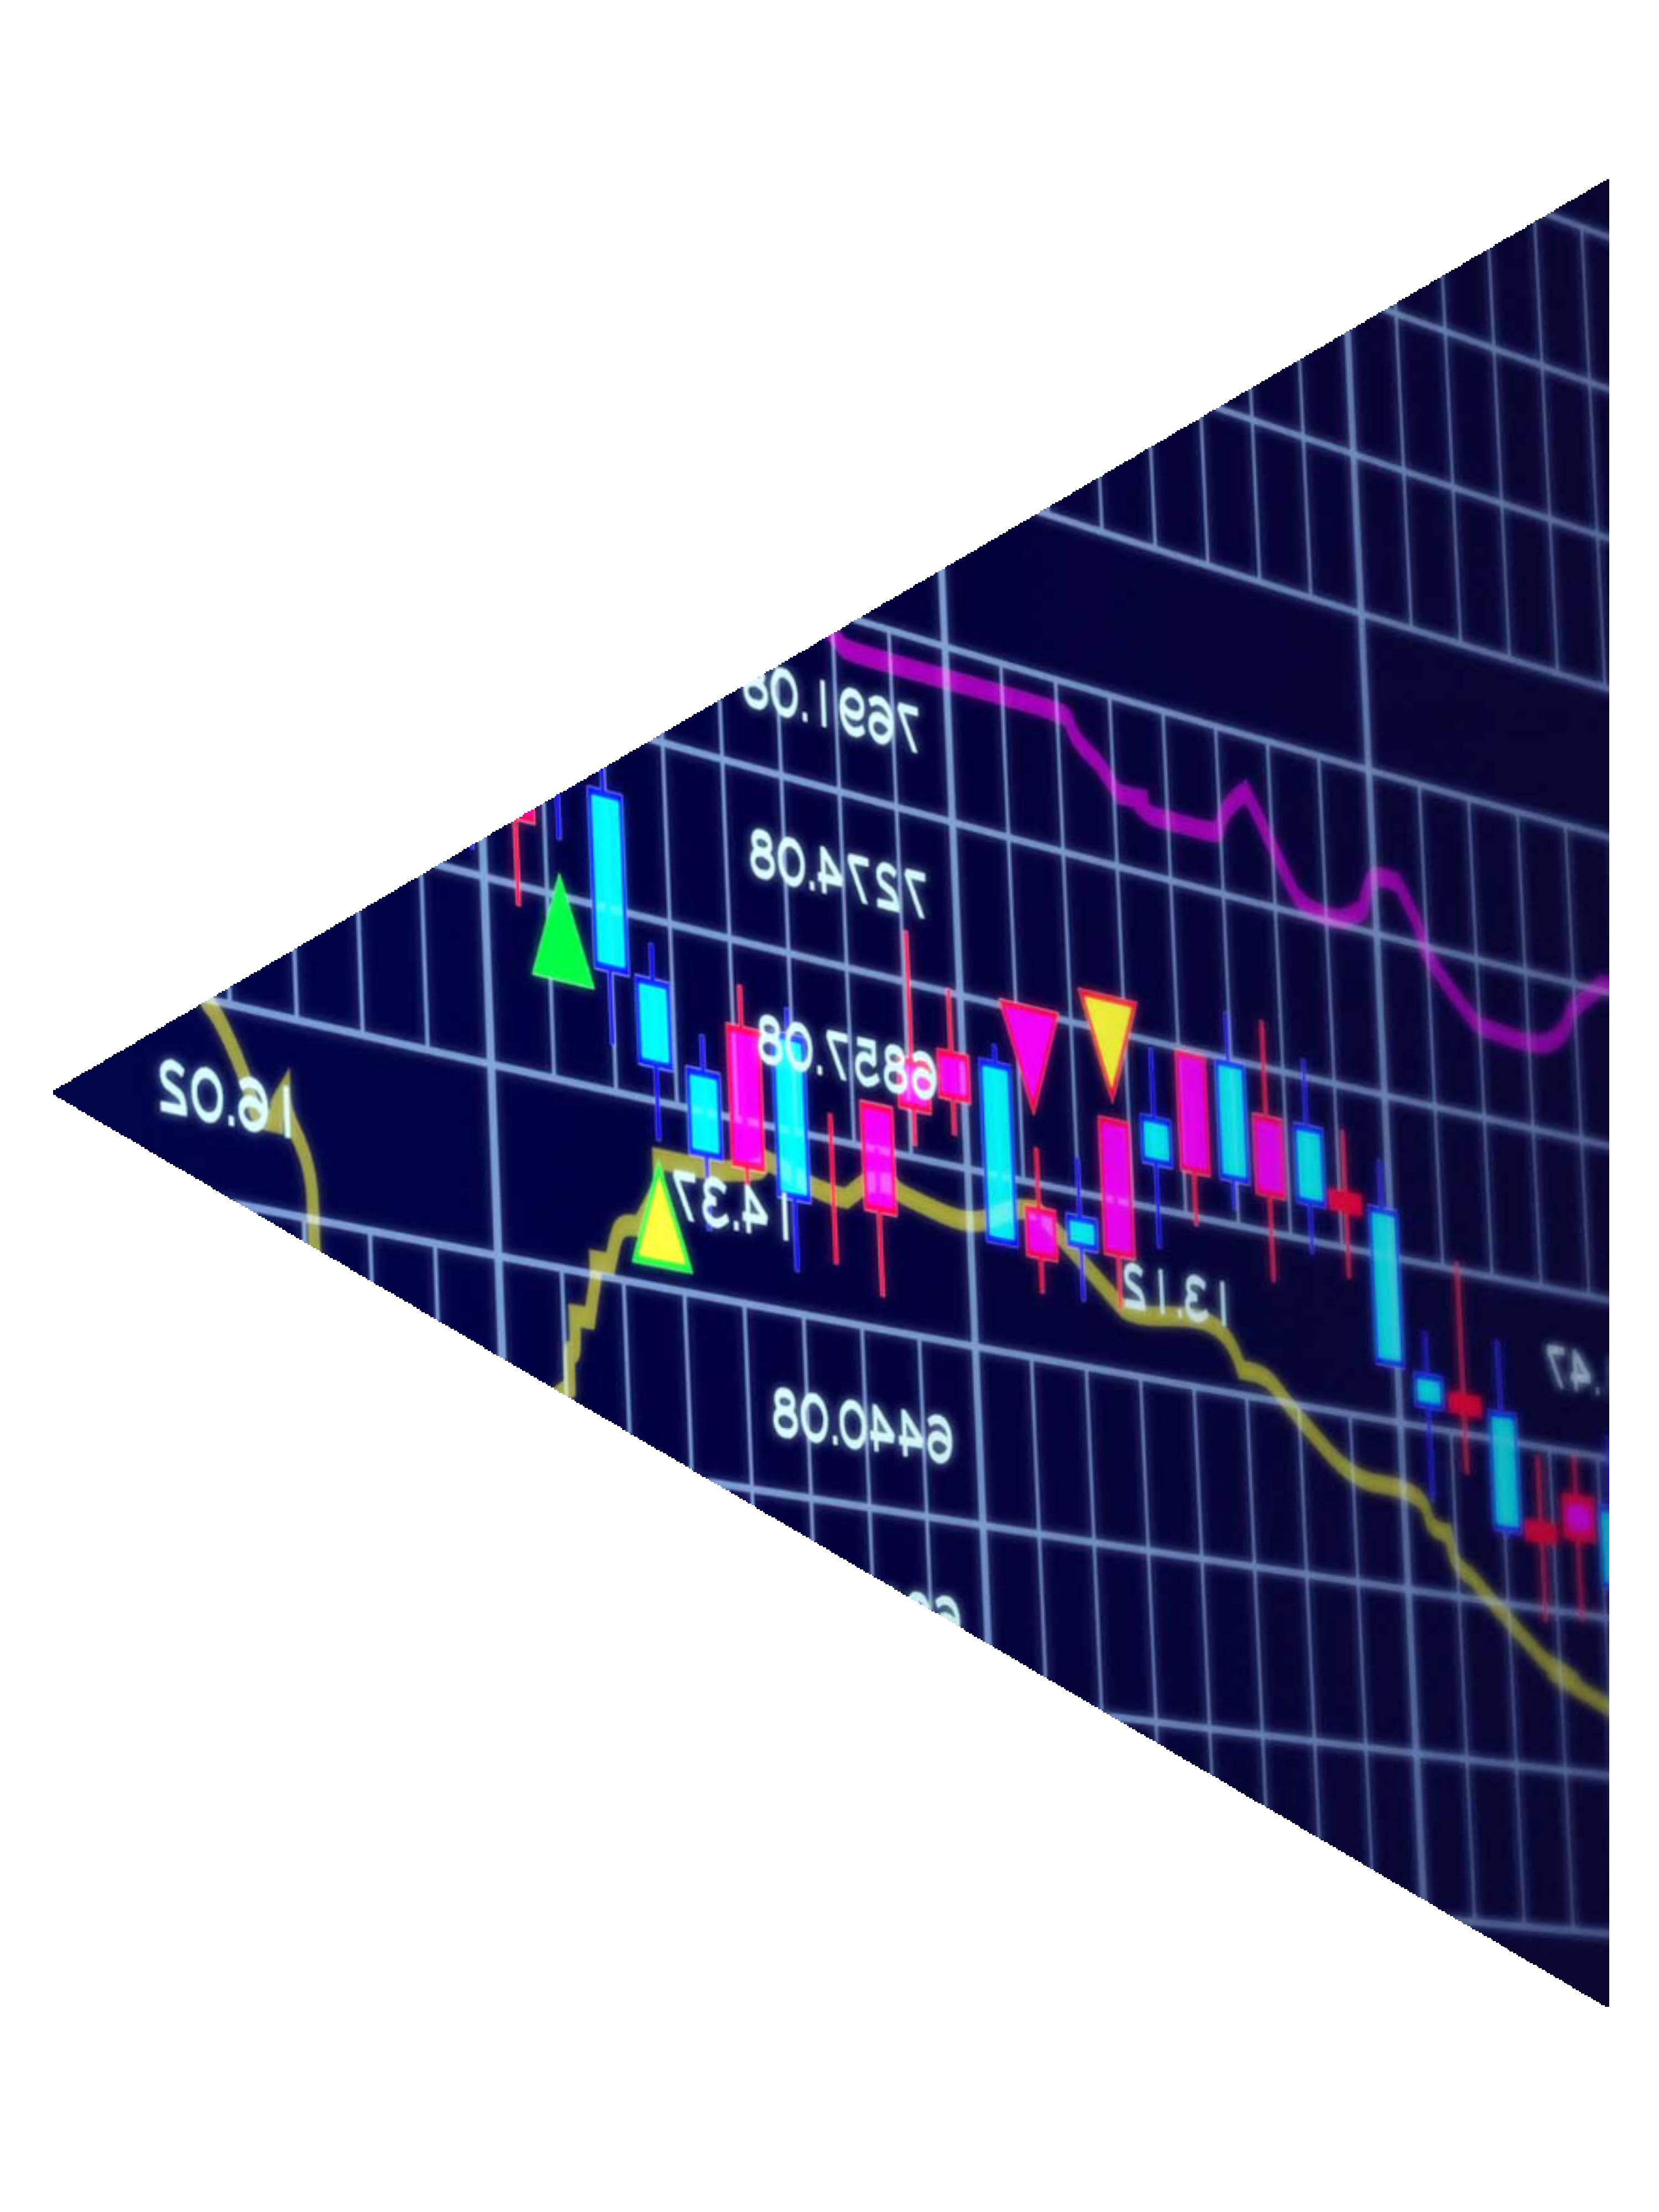
\includegraphics[width=22cm]{triangle.png}};
	\fill [jaune] (14,5) -- (2.5, 12) -- (20,25) -- (14, 20);
 \end{tikzpicture}}


\SetBgContents{\MyGraphicLogo}% Select included image

\SetBgPosition{current page.north west}% Select location
\SetBgOpacity{1.0}% Select opacity
\SetBgAngle{0.0}% Select roation of logo
\SetBgScale{1.0}% Select scale factor of logo


\usepackage{listings}
\usepackage{color}

\definecolor{mygreen}{rgb}{0,0.6,0}
\definecolor{mygray}{rgb}{0.5,0.5,0.5}
\definecolor{mymauve}{rgb}{0.58,0,0.82}

\lstset{ 
  backgroundcolor=\color{white},   % choose the background color; you must add \usepackage{color} or \usepackage{xcolor}; should come as last argument
  basicstyle=\footnotesize,        % the size of the fonts that are used for the code
  breakatwhitespace=false,         % sets if automatic breaks should only happen at whitespace
  breaklines=true,                 % sets automatic line breaking
  captionpos=b,                    % sets the caption-position to bottom
  commentstyle=\color{mygreen},    % comment style
  deletekeywords={...},            % if you want to delete keywords from the given language
  escapeinside={\%*}{*)},          % if you want to add LaTeX within your code
  extendedchars=true,              % lets you use non-ASCII characters; for 8-bits encodings only, does not work with UTF-8
  frame=single,	                   % adds a frame around the code
  keepspaces=true,                 % keeps spaces in text, useful for keeping indentation of code (possibly needs columns=flexible)
  keywordstyle=\color{blue},       % keyword style
  language=Octave,                 % the language of the code
  morekeywords={*,...},            % if you want to add more keywords to the set
  numbers=left,                    % where to put the line-numbers; possible values are (none, left, right)
  numbersep=5pt,                   % how far the line-numbers are from the code
  numberstyle=\tiny\color{mygray}, % the style that is used for the line-numbers
  rulecolor=\color{black},         % if not set, the frame-color may be changed on line-breaks within not-black text (e.g. comments (green here))
  showspaces=false,                % show spaces everywhere adding particular underscores; it overrides 'showstringspaces'
  showstringspaces=false,          % underline spaces within strings only
  showtabs=false,                  % show tabs within strings adding particular underscores
  stepnumber=2,                    % the step between two line-numbers. If it's 1, each line will be numbered
  stringstyle=\color{mymauve},     % string literal style
  tabsize=2,	                   % sets default tabsize to 2 spaces
  title=\lstname                   % show the filename of files included with \lstinputlisting; also try caption instead of title
}



%%%%%%%%%%%%%%%%%%%%%%%%%%%%%%%%%%%%%%%%%%%%%%%%%%%%%%%%%%%%%%%%%%%%
%																																	   %
%																																	   %
%																																	   %
%										Informations générales sur le document															   %
%																																	   %
%																																	   %
%%%%%%%%%%%%%%%%%%%%%%%%%%%%%%%%%%%%%%%%%%%%%%%%%%%%%%%%%%%%%%%%%%%%

 \usepackage{fontspec}
  \usepackage[bold-style=upright]{unicode-math}
  \defaultfontfeatures{Scale=1}
  \setmainfont[Ligatures=TeX,Numbers=OldStyle]{Lucida Bright OT}
  \setmathfont[RawFeature=+ss04]{Lucida Bright Math OT}
  \setsansfont[Scale=1.0,Numbers=OldStyle]{Myriad Pro}
  \newfontfamily\fullcaps[Letters=Uppercase,Numbers=Uppercase]{Myriad Pro}
  \usepackage[babel=true]{microtype}
  \usepackage{icomma}
  
  \usepackage{amsmath,amsfonts,amssymb,amsthm,epsfig,epstopdf,titling,url,array}
  \theoremstyle{definition}
\newtheorem{defn}{Definition}[section]
  
  
  
  
  
  
  
  
  
\title{Implied volatility}
\author{Maxence COUPET}
\date{March 2018}



\MHInternalSyntaxOn
\MH_set_boolean_T:n {outer_mult}
\MHInternalSyntaxOff

\newenvironment{nalign}{
    \begin{equation}
    \begin{aligned}
}{
    \end{aligned}
    \end{equation}
    \ignorespacesafterend
}
%%%%%%%%%%%%%%%%%%%%%%%%%%%%%%%%%%%%%%%%%%%%%%%%%%%%%%%%%%%%%%%%%%%%
%																																	   %
%																																	   %
%																																	   %
%												Mis en page du document																   %
%																																	   %
%																																	   %
%%%%%%%%%%%%%%%%%%%%%%%%%%%%%%%%%%%%%%%%%%%%%%%%%%%%%%%%%%%%%%%%%%%%


\begin{document}
	\selectlanguage{french}
	% page de garde
	\pagenumbering{gobble}
	\maketitle
	\newpage
	% début du rapport
	
	
	


\newcommand{\MyGraphicLog}{% For imported graphic logo
\begin{tikzpicture}[remember picture,overlay,yshift=-15cm, xshift=10.5cm]
\definecolor{jaune}{RGB}{16, 52, 78};
\fill[jaune] (-11, -16) -- (13, -16) -- (13, -12.1) -- (-11, -12.1);
 \end{tikzpicture}}


\SetBgContents{\MyGraphicLog}% Select included image


\SetBgPosition{current page.north west}% Select location
\SetBgOpacity{1.0}% Select opacity
\SetBgAngle{0.0}% Select roation of logo
\SetBgScale{1.0}% Select scale factor of logo

\pagestyle{fancy}
\renewcommand\headrulewidth{0pt}
\lhead{}\chead{}\rhead{}
\cfoot{\vspace*{6\baselineskip} \textcolor{white}{\thepage} \large}
	\newpage

	\pagenumbering{arabic}

%%%%%%%%%%%%%%%%%%%%%%%%%%%%%%%%%%%%%%%%%%%%%%%%%%%%%%%%%%%%%%%%%%%%
%																																	   %
%																																	   %
%																																	   %
%								Début du document (commencez à taper votre texte ici)													   %
%																																	   %
%																																	   %
%%%%%%%%%%%%%%%%%%%%%%%%%%%%%%%%%%%%%%%%%%%%%%%%%%%%%%%%%%%%%%%%%%%%

\section{Different volatilities}

One must be aware of the differences between realized volatility and implied volatility. In most cases, when a market participant says ''volatility'' we must understand implied volatility.


\subsection{Realized volatility}

The realized volatility (or historical volatility) is the standard deviation of the logarithmic returns of an underlying. Let's consider $N$ historical prices for an underlying at different times $t_i$. The return will then be :
$$r_i = ln\left( \frac{S(t_i)}{S(t_{i-1})}\right)$$
Note that we could also have taken the return as the percentage change in each period. The mean of returns will be :
$$\bar{r}=\frac{1}{N} \sum_{i=1}^N r_i$$
and an unbiaised estimate of the standard deviation would be :
$$ \sigma = \sqrt{\frac{1}{N-1}\sum_{i=1}^N (r_i - \bar{r})^2}$$

A very important point with volatility is that it is always expressed as annualized volatility. So you will have to multiply this annualized volatility with the good time frame. For exemple, if we have a volatility $\sigma =20\%$ for a stock, the daily volatility is $\frac{\sigma}{\sqrt{252}} \approx 1.3 \%$. The value 252 represent the number of trading days in a year and is a common convention for the number of days in a year.

When we focus on realized volatility, we must keep in mind that the historical period has to be chosen very carefully since the historical data is not a good indicator of future performances in most cases.

\newpage
\subsection{Implied volatility}

When using the historical volatility, we only have information about the past evolution of the underlying's volatility, we do not have any information about the current market sentiments and forecasting. This is what implied volatility intend to do. In order to compute implied volatility, we have to find very liquid derivatives, such as vanilla options. We then have a market price for the derivative, one price that all market participants agreed on. We can now use the Black-Scholes explicit formula, in order to find the volatility which would lead to the market price, this volatility is called the implied volatility. It is the market consensus on the futur value of the volatility. While they are often close, implied volatility and historical volatility are typically not equal. 

If we note $P_{BS}(\sigma)$ the price given by the Black-Scholes formula, considering all parameters constant except the volatility, and $P_{market}$ the price observed on the market for the same derivative, computing implied volatility is the same as resolving the following equation :
$$ (E) : \quad \sigma \in \mathbb{R}^+, \; P_{BS}(\sigma) = P_{market} $$

Unfortunatly, we can not invert the Black-Scholes fomula to get the volatility. We then have to use a numerical method to solve the previous equation. One of the method that could be used is the Newton-Raphson algorithm as presented with an application in python in the \href{sec:iv_calculus}{annexe} of this document, but it is a rather simple method.

With this method, volatility is just an interpretation of the price of the derivative and most market participants will talk about buying certain amount of volatility instead of buying at a certain price, since it is the same information, but the value of volatility is more useful than the derivative's price for hedging considerations.

One important property of the implied volatility is that it is the same for calls and puts, therefore it does not matter if we compute it with calls or puts. This proprety comes from the call-put parity, which does not make any assumption except the arbitrage-free hypothesis, thus we can apply this property to both market prices and the Black-Scholes prices :
$$ c_{BS} - p_{BS} = S_0 - K e^{-rT}$$
$$c_{market} - p_{market} = S_0 - K e^{-rT}$$

Thus we have :
$$c_{market} - c_{BS} = p_{market} - p_{BS}$$

So the approximation of pricing is exactly the same for calls and puts.

\newpage
\section{Volatility surface}
One interesting property of implied volatility, is something that the Black-Scholes model does not predict : the implied volatility has different values across strikes and also across maturities, as we can see in figures \ref{fig:skew} and \ref{fig:skew_term_structure}.

 When we fix the maturity of the option, and look at different values of implied volatility for different strikes, we are getting the volatility skew (or smile). When we fix the strike price (usually to the spot), and look at different values of implied volatility for different maturities, we are getting the volatility term structure. When we fix neither the strike nor the maturity, we are getting a 2D plotting of the volatility, called the volatility surface.
 
\subsection{Volatility skew}

\subsubsection{Presentation}

As of now, we will not use explicit value for the strike of an option, but rather a percentage (ex : if the underlying price is 50\$ and the strike is 55\$, we will have a strike of 110\%), this is called the moneyness. This notation is also very popular among market participants. 



\begin{figure}[!h]
	\centering
	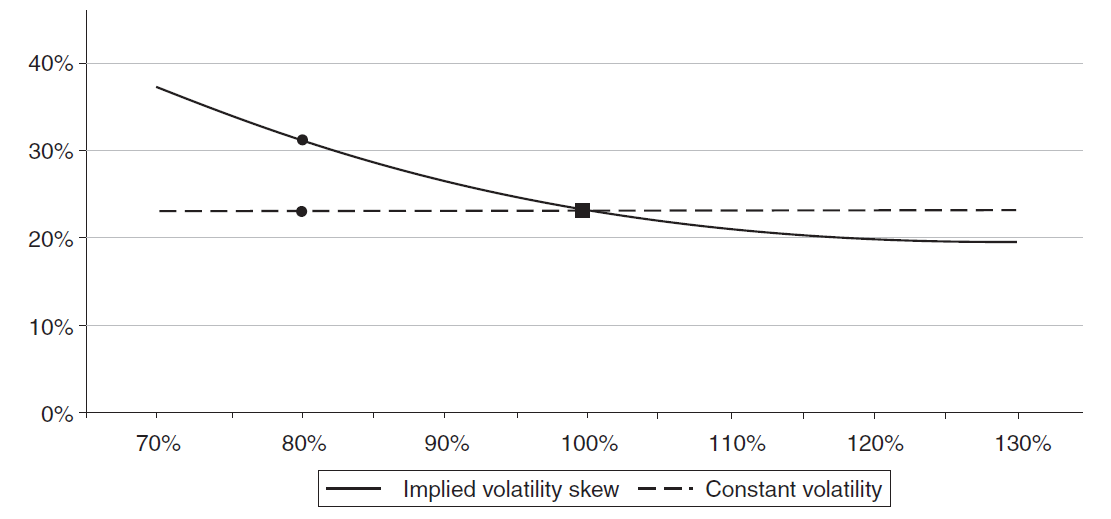
\includegraphics[width=\textwidth]{skew.png}
    \caption{Volatility skew and flat volatility across strikes}
    \label{fig:skew}
    \end{figure}
    
    The implied volatility across different strikes can take several shapes, depending of the underlying, but they could be classified in two main shapes : skew and smile. The skew is represented with a flat volatility in figure \ref{fig:skew}. We can see that it tends to overvalue volatility (therfore the price) of ITM calls and OTM puts, but it also tends to undervalue volatility for OTM calls and ITM puts. The skew shape implies that the volatility will be higher for downward movement than for upward movement. If we think about the log-normal distrubution of returns, it also means that tails will be more important for downward movement, and less important for upward movement, as illustrated in figure \ref{fig:skew_density}. Empirically, this new density is a much better approximation than the log-normal density, for some underlyings.
    
    \begin{figure}[!h]
	\centering
	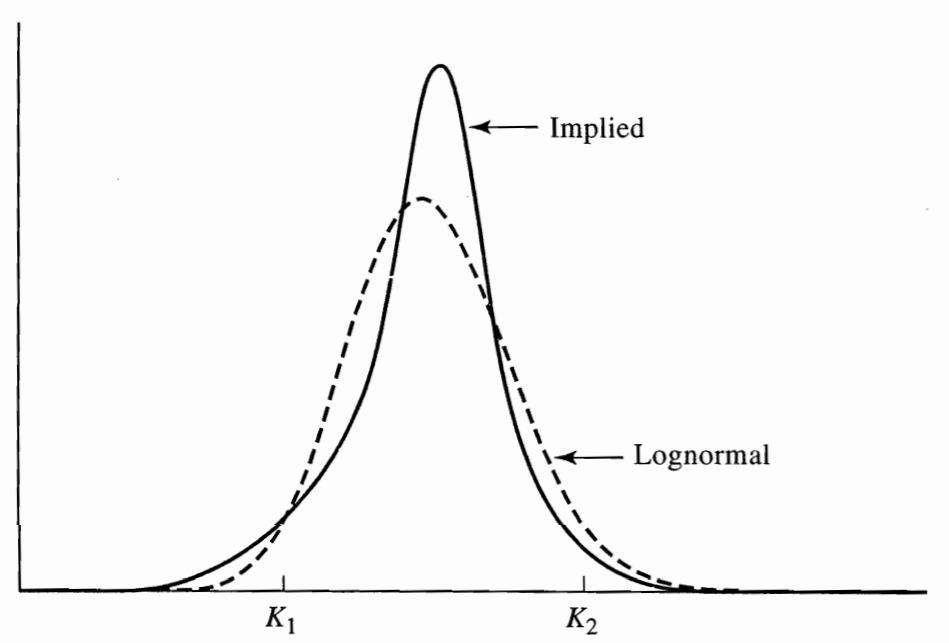
\includegraphics[width=\textwidth]{skew_density.png}
    \caption{Skew implied density and log-normal density}
    \label{fig:skew_density}
    \end{figure}
    
    The skew will be in most cases the shape of implied volatility for stocks. The fact of overvaluing OTM puts for stocks could be explained by the fact that market participants tend to buy more protection for a downward movement than for upward movement on the equity market, this means that market participants fear a downward tread on the equity market. Another explaination for the skew is that when a company suffer losses, its capital has a higher leverage and thus shares of this company will have a higher volatility. Empirically, the fact that OTM puts are overvalued lead to a very expensive cost of hedging in a decreasing market.
    \newline
    
    The smile has a different shape, and is common in the commodity or foreign exchange market, since they are both market with important mean reversal property (if a currency is too high with respect to another currency, it will loose any interest since it is too expensive, so it will loose value and thus return to its mean). Figure \ref{fig:smile} shows the shape of a volatility smile :
    
    \begin{figure}[!h]
	\centering
	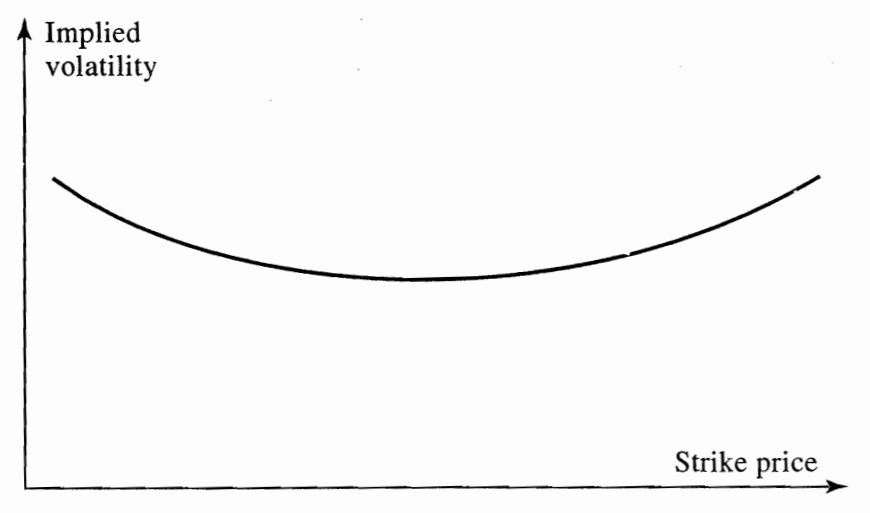
\includegraphics[width=0.9\textwidth]{smile.png}
    \caption{Volatility smile}
    \label{fig:smile}
    \end{figure}
    
    
    
    We can see that both ITM and OTM options will have higher volatility and thus will be overvalued with a smile shape, which will lead to heavier tails than with the log-normal distribution (this means that the kurtosis (fourth moment) will be higher), as we can see on figure \ref{fig:smile_density} :
    
     \begin{figure}[!h]
	\centering
	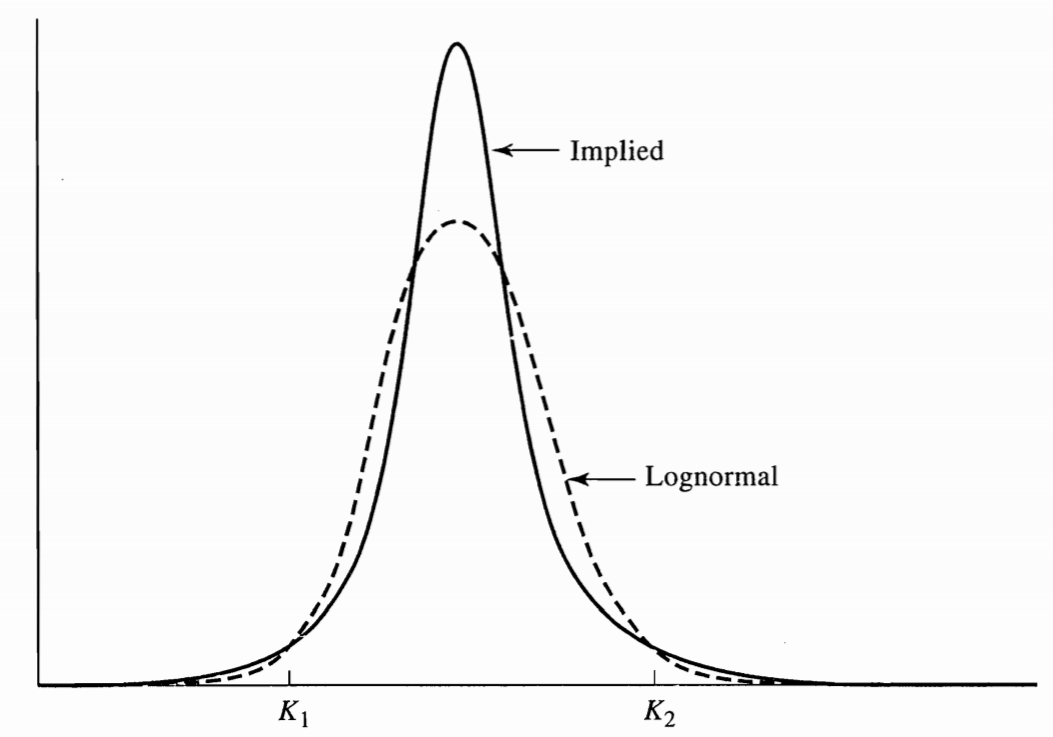
\includegraphics[width=0.9\textwidth]{smile_density.png}
    \caption{Smile implied density and log-normal density}
    \label{fig:smile_density}
    \end{figure}
    
    
    There is one more known shape for the skew (but quite rare), when we are expecting some very important news about one stock. In this case, we could consider that the stock can only go up of a certain quantity or go down of another certain quantity. The probability density will then be the sum of two log-normal laws, as on figure \ref{fig:skew_binom_density.png} :
      \begin{figure}[!h]
	\centering
	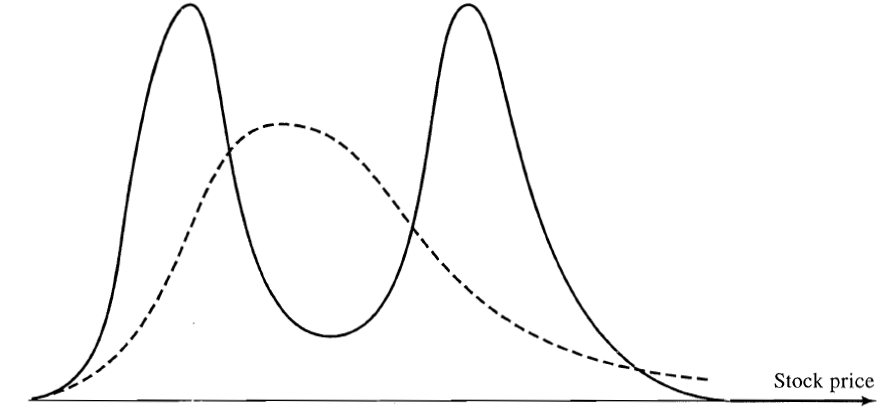
\includegraphics[width=0.9\textwidth]{skew_binom_density.png}
    \caption{Bimodal implied density and log-normal density}
    \label{fig:skew_binom_density}
    \end{figure}
    
    The implied volatility will then have the shape described on figure \ref{fig:skew_binom}. Keep in mind that it is more a theorical shape for an extreme scenario, that an empirically observed shape.
    \begin{figure}[!h]
	\centering
	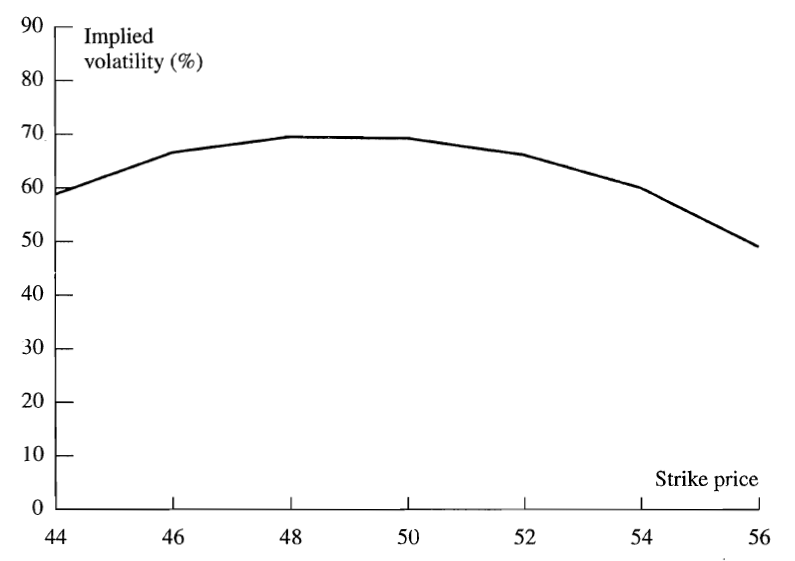
\includegraphics[width=0.9\textwidth]{skew_binom.png}
    \caption{Bimodal implied volatility}
    \label{fig:skew_binom}
    \end{figure}
   
   \subsubsection{Computing and trading the skew}
   As skew, we mean the slope of the volatility skew. So one important point is to know where to compute this slope. Usually, we compute the skew arround the ATM price in order to give an indication of the position of skew volatility. A mathematical definition of the skew could be :
   $$ skew = \frac{\partial \sigma_{implied}(K)}{\partial K}$$
   
   But in most cases we will use the 90\% and 100\% strike prices in order to compute the skew :
   $$ skew = \frac{\sigma_{implied}(100\%) - \sigma_{implied}(90\%)}{10\%} $$
   
   Figure \ref{fig:skews} represents volatility skews with different skews. We say that one volatility is more skewed than another if its skew is more important in absolute value and thus is the volatility skew is steeper.
   
   \begin{figure}[!h]
	\centering
	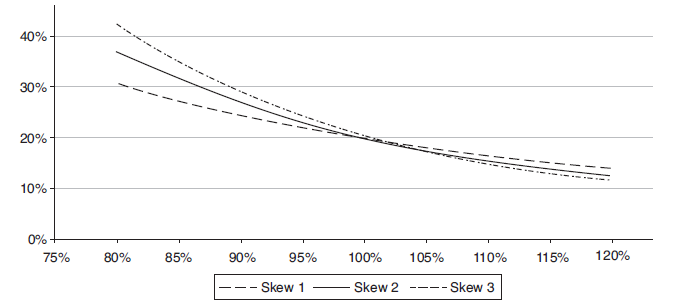
\includegraphics[width=0.9\textwidth]{skews.png}
    \caption{Implied volatilities with different skews}
    \label{fig:skews}
    \end{figure}
    
    When involved in a trade dealing with options with different strikes, one market participant should be aware of the skew and the consequencies of an increase or decrease of skew, otherwise his pricing would not be accurate since the hedging cost taken into account is not the real one.
    
    One simple strategy to trade (or hedge) the skew is a vertical spread. For example, let's consider that one market participant thinks that the skew will be steeper that it is today, he would like to be long the skew. This could be done by taking a long position in a bull spread (long a 90\% call and short a 100\% call). Indeed if the skew is steeper, the implied volatility of the 90\% call will be higher and the implied volatility of the 100\% call will be lower, thus the price of the 90\% call (which we are long) will be higher and the price of the 100\% call (which we are short) will be lower and the value of the bull spread will be more important.
    
    An intersting property of the skew for equities is that the skew of an index is steeper than the skew of individual stocks. This property is the consequency of a rise of the correletation between stocks when a market decline : an imporant decrease of an index means that a majority of the stocks are declining, thus this means an increasing correlation between individual stocks and finally an increase of the volatility of the index. This property is useful when we consider cross-hedging (hedging with another underlying that the underlying of the derivative we want to hedge). Cross-hedging is used for liquidity concerns, if a derivative has not an important market volume, one would prefer to hedge with a more liquid derivative (for which he could computethe implied volatility, remember that we can only compute implied volatility for very liquid derivatives). Since derivatives for single stocks might not be very liquid, one often preffer to hedge with derivative on stock indexes and thus one should be aware of the difference of skew between indexes and single stocks in order to adjust his hedging positions.
    
    
   \newpage
   \subsection{Volatility skew's convexity}
   As for the greek of an option, when one wants to observe sensitivity with respect to a parameter for an important variation, he should use higher degree of derivative. The skew's convexity is the curvature of the skew, it gives us an information about how fast the skew may change. As for the skew itself, the skew's convexity could be defined by a mathematical formula :
   $$\text{skew's convexity} = \frac{\partial^2 \sigma_{implied}(K)}{\partial K^2}$$
   
   But we will also prefer a formula given by the finite differences method, for the 90\%, 100\% and 110\% strikes calls :
   $$\text{skew's convexity} = \frac{\sigma_{implied}(90\%) - 2 \sigma_{implied}(100\%) + \sigma_{implied}(110\%)}{1\%}$$
   Figure \ref{fig:skew_convexity} represent volatilities with the same skew but different convexities :
   \begin{figure}[!h]
	\centering
	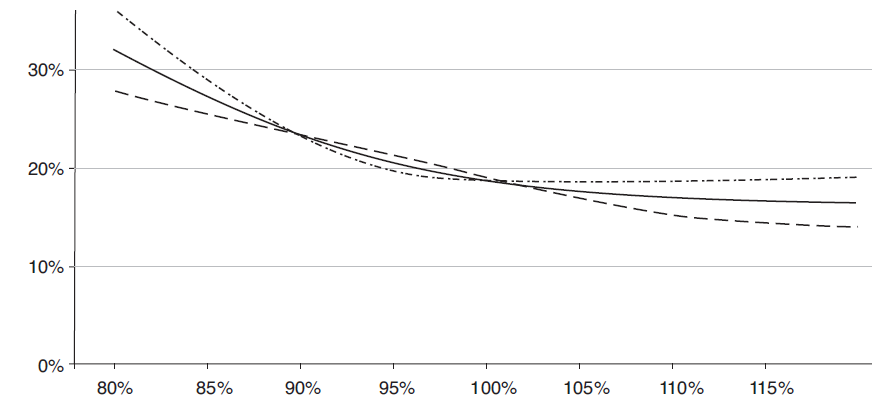
\includegraphics[width=0.9\textwidth]{skew_convexity.png}
    \caption{Different skew's convexity}
    \label{fig:skew_convexity}
    \end{figure}
    
   Since the computation of the skew's convexity involve three different strikes, it seams logical to use option combinaisons also involving three different strikes in order to trade (or hedge) the skew's convexity. 
   
   Let's assume that one thinks that the skew's convexity will increase in the future, thus he wishes to be long the skew's convexity. This could be done by entering a long butterfly spread. Indeed, if we long a 90\%-100\%-110\% butterfly spread, which means that we long one 90\% call, we short two 100\% call and finally long one 110\% call, an increase in the skew's convexity will increase the volatility of both 90\% and 110\% strikes but will decrease the value of the 100\% strike, which will increase the value of our long butterfly spread.
   
   Another interesting property of the skew's convexity is for equities : the skew's convexity of an index is lower that the one of a single stock. This is because an important moove in volatility will have more impact on a single that on a index, since the index is (partially) diversified.
   \newpage
   \subsection{Volatility term structure}
   
   \newpage
\appendix
\section{Computation of implied volatility}
\label{sec:iv_calculus}

In order to compute the implied volatility, we need some market data. We provide with this file few datas downloaded on Reuters for calls on the S\&P 500 with a maturity of one month. As risk-free rate we will use the one month LIBOR rate and will use a prediction for the continuously compounded dividend rate. After getting prices, we use the scipy implementation of the Newton-Raphson method, with an error function for our equation (since we have to transform it to be an equation of the type : $(E): \quad f(x) = 0$). As first approximation for the Newton-Raphson method, we give the annualized historical volatility of the previous month. The result is given by figure \ref{fig:sp_iv} :

\begin{figure}[!h]
	\centering
	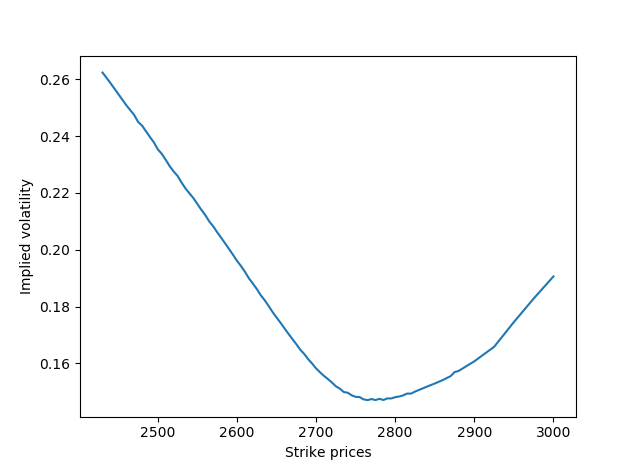
\includegraphics[width=0.9\textwidth]{SP500_iv.png}
    \caption{S\&P 500 implied volatility for one month maturity}
    \label{fig:sp_iv}
    \end{figure}
    
    As we can see, the minimum of volatility (2760 \$) is far from the spot price (2600 \$) and the forward price (2604 \$). This means that market participants are forecasting a value arround 2760 \$ for the S\&P 500.
   
    The python code is the following :
    
    \lstinputlisting[language=Python]{implied_volatility.py}
\end{document}